\documentclass[12pt]{article}
\usepackage[margin=1in]{geometry} 
\usepackage{amsmath}
\usepackage{tcolorbox}
\usepackage{amssymb}
\usepackage{amsthm}
\usepackage{lastpage}
\usepackage{fancyhdr}
\usepackage{accents}
\pagestyle{fancy}
\setlength{\headheight}{40pt}


\newenvironment{solution}
  {\renewcommand\qedsymbol{$\blacksquare$}
  \begin{proof}[Solution]}
  {\end{proof}}
\renewcommand\qedsymbol{$\blacksquare$}

\newcommand{\ubar}[1]{\underaccent{\bar}{#1}}

\begin{document}

% Cover Page
\begin{titlepage}
  \centering
  
  {\scshape\LARGE University of British Columbia \par}
  \vspace{1cm}
  {\scshape\Large CPSC 425: Computer Vision\par}
  \vspace{1.5cm}
  {\huge\bfseries Assignment 1\par}
  \vspace{2cm}
  {\Large\itshape Simon Ghyselincks\par}
  \vfill
  Self-Studied based off of UBC CPSC 425 2023T1 course material\par

  \vfill

  % Bottom of the page
  {\large 2021\par}
\end{titlepage}

\lhead{UBC CPSC 425 Computer Vision: Assignment 1} 
\rhead{Term II 2020} 
\cfoot{\thepage\ of \pageref{LastPage}}



\lhead{UBC CPSC 425 Computer Vision: Assignment 1} 
\rhead{Term II 2020} 
\cfoot{\thepage\ of \pageref{LastPage}}

\noindent In this question, you will be practicing filtering by hand on the following image. You will enter your final result for each question in the provided empty tables.

\begin{center}
\begin{tabular}{|l|l|l|l|l|}
\hline
1 & 0 & 0 & 0 & 1 \\ \hline
2 & 3 & 0 & 8 & 0 \\ \hline
2 & 0 & 0 & 0 & 3 \\ \hline
0 & 0 & 1 & 0 & 0 \\ \hline
\end{tabular}
\end{center}
\textbf{Note that you do not have to fill all the cells. If a cell contains a number that is not an integer, enter it as a fraction.}

\subsection*{Question (1a)} Apply the correlation filter to the image with \textbf{no padding}.
\begin{center}
\begin{tabular}{|c|c|c|}
\hline
0  & 0 & 1 \\ \hline
0  & 0 & 0 \\ \hline
-1 & 0 & 0 \\ \hline
\end{tabular}
\end{center}

\noindent Enter your final result here in integer or fraction:

\begin{center}
\begin{tabular}{|l|l|l|l|l|}
\hline
\hspace{1mm} & \hspace{1mm} & \hspace{1mm} & \hspace{1mm} & \hspace{1mm} \\ \hline
\hspace{1mm} & -2 \hspace{1mm} & 0 \hspace{1mm} & 1 \hspace{1mm} & \hspace{1mm} \\ \hline
\hspace{1mm} & 0 \hspace{1mm} & 8 \hspace{1mm} & -2 \hspace{1mm} & \hspace{1mm} \\ \hline
\hspace{1mm} & \hspace{1mm} & \hspace{1mm} & \hspace{1mm} & \hspace{1mm} \\ \hline
\end{tabular}
\end{center}

\subsection*{Question (1b)} Apply the convolution filter to the image with \textbf{no padding}.
\begin{center}
\begin{tabular}{|c|c|c|}
\hline
0  & 0 & 1 \\ \hline
0  & 0 & 0 \\ \hline
-1 & 0 & 0 \\ \hline
\end{tabular}
\end{center}

\noindent Enter your final result here in integer or fraction:

\begin{center}
\begin{tabular}{|l|l|l|l|l|}
\hline
\hspace{1mm} & \hspace{1mm} & \hspace{1mm} & \hspace{1mm} & \hspace{1mm} \\ \hline
\hspace{1mm} & 2 \hspace{1mm} & 0 \hspace{1mm} & -1 \hspace{1mm} & \hspace{1mm} \\ \hline
\hspace{1mm} & 0 \hspace{1mm} & -8 \hspace{1mm} & 2 \hspace{1mm} & \hspace{1mm} \\ \hline
\hspace{1mm} & \hspace{1mm} & \hspace{1mm} & \hspace{1mm} & \hspace{1mm} \\ \hline
\end{tabular}
\end{center}

\newpage

\subsection*{Question (1c)} Apply the filter to the image with \textbf{zero padding} (zero padding means to pad your image with zeros; it is not the same as ``no padding").
\begin{center}
\begin{tabular}{|c|c|c|}
\hline
1/9  & 1/9 & 1/9 \\ \hline
1/9  & 1/9 & 1/9 \\ \hline
1/9  & 1/9 & 1/9 \\ \hline
\end{tabular}
\end{center}

\noindent Enter your final result here in integer or fraction:

\begin{center}
\begin{tabular}{|l|l|l|l|l|}
\hline
\hspace{1mm} $\frac{6}{9}$ & \hspace{1mm} $\frac{6}{9}$& \hspace{1mm}$\frac{11}{9}$ & \hspace{1mm} $\frac{9}{9}$& \hspace{1mm}$\frac{9}{9} $\\ \hline
\hspace{1mm} $\frac{8}{9}$ & \hspace{1mm} $\frac{8}{9}$& \hspace{1mm}$\frac{11}{9}$ & \hspace{1mm} $\frac{12}{9}$& \hspace{1mm}$ \frac{12}{9}$\\ \hline
\hspace{1mm} $\frac{7}{9}$& \hspace{1mm} $\frac{8}{9}$& \hspace{1mm}$\frac{12}{9}$ & \hspace{1mm} $\frac{12}{9} $& \hspace{1mm}$ \frac{11}{9}$\\ \hline
\hspace{1mm} $\frac{2}{9}$ & \hspace{1mm} $\frac{3}{9}$ & \hspace{1mm}$\frac{1}{9}$ & \hspace{1mm} $\frac{4}{9}$& \hspace{1mm}$ \frac{3}{9}$\\ \hline
\end{tabular}
\end{center}

\section*{Part 2}

\subsection*{1.}
Box filters for 3,4,5
\\
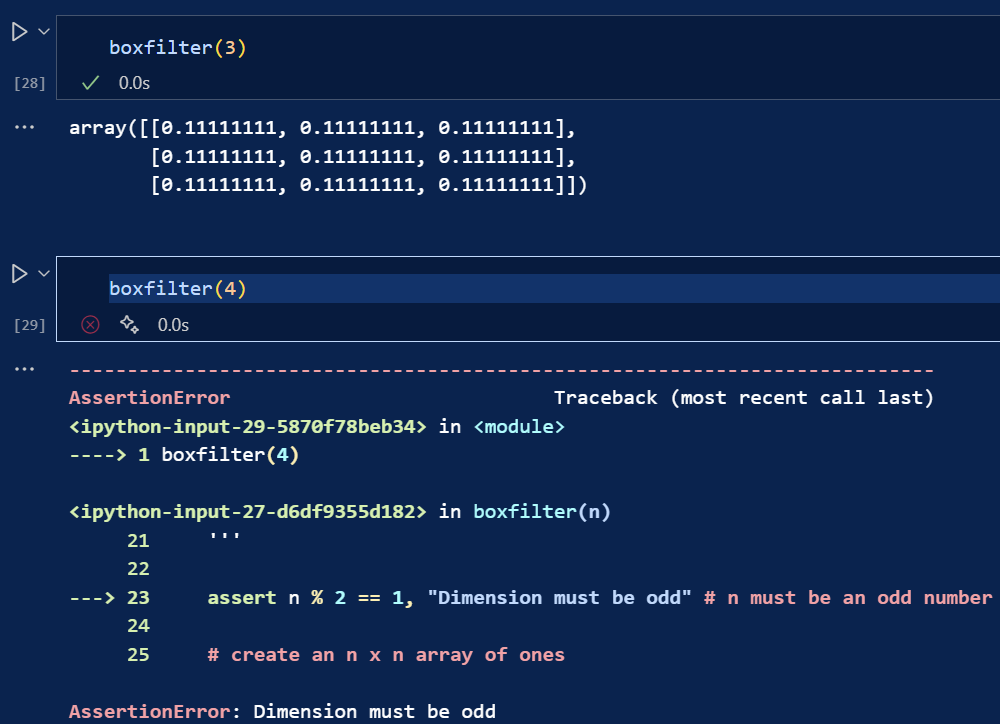
\includegraphics[width=0.65\textwidth]{imgs/1-1.png}\\
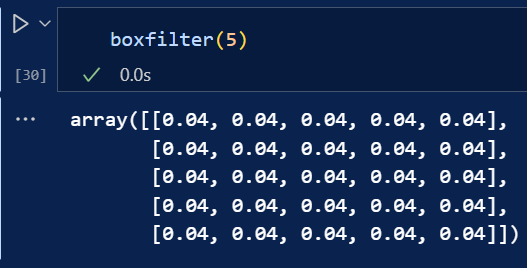
\includegraphics[width=0.65\textwidth]{imgs/1-2.png}
\subsection*{2.}
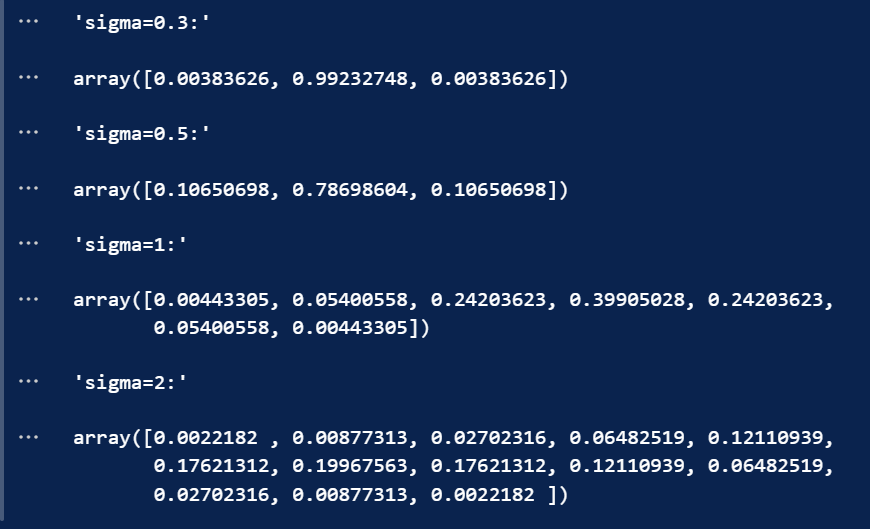
\includegraphics[width=0.65\textwidth]{imgs/2-1.png}
\subsection*{3.}
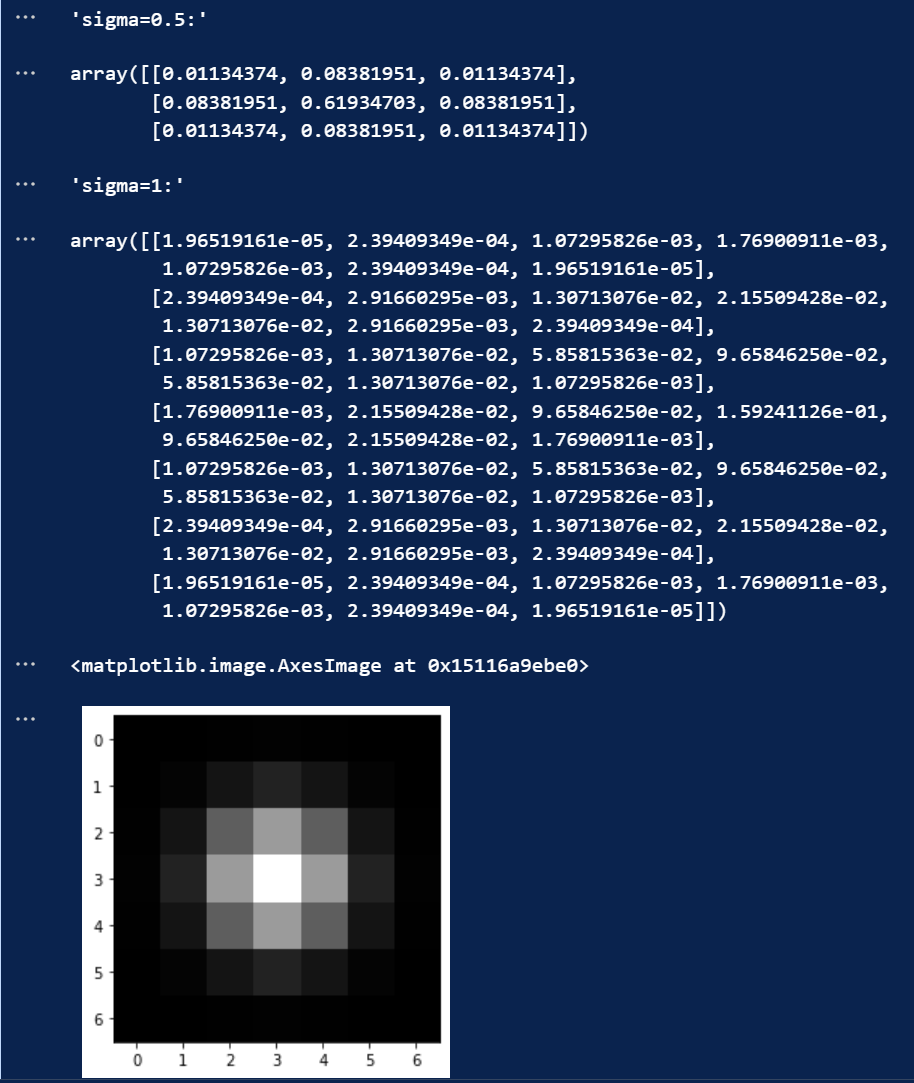
\includegraphics[width=0.65\textwidth]{imgs/3-1.png}
\subsection*{4.}
A comparison of before and after dog picture\\
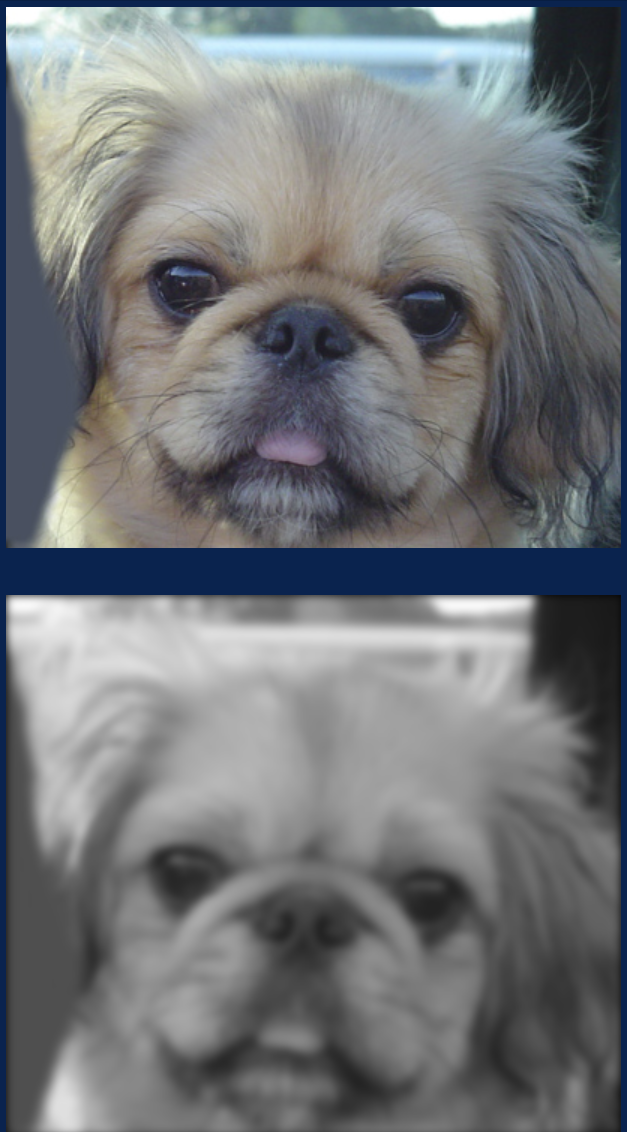
\includegraphics[width=0.65\textwidth]{imgs/4-d.png}

\subsection*{5.}
There are two different functions because they are not equivalent. The correlation and convolution are only the same for a 180 degree rotationally symmetric kernel, which is true for the Gaussian. Rotating the kernel by 180 still gives the same result.

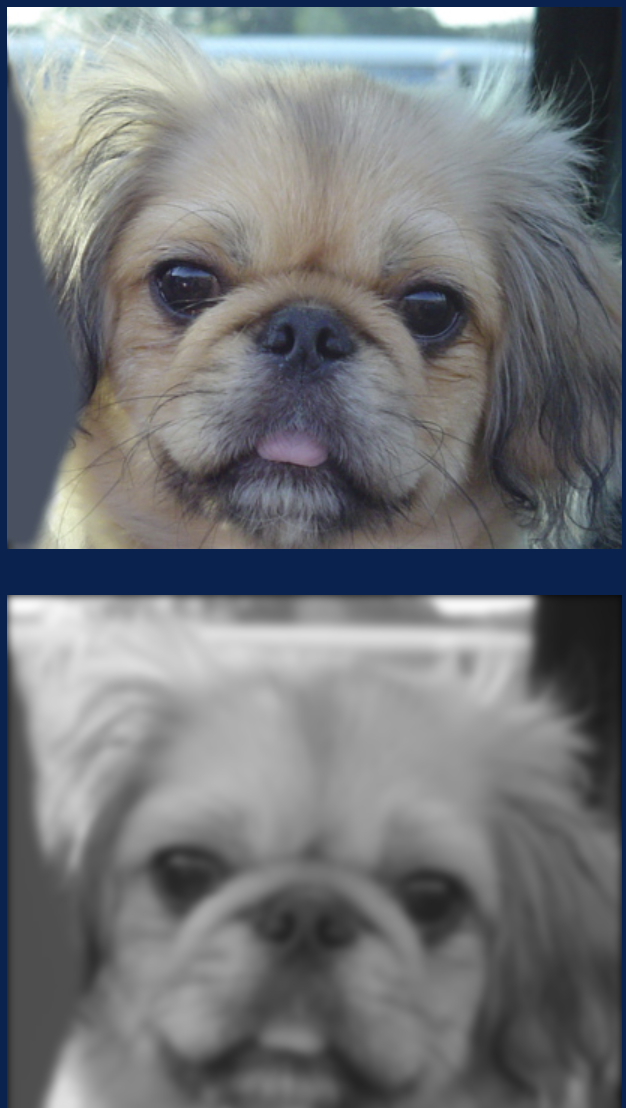
\includegraphics[width=0.65\textwidth]{imgs/5-c.png}

\subsection*{6.}
Manual method takes 0.8032005310058594 seconds\\
Scipy method takes 0.7100874423980713 seconds

The scipy method is faster, likely because it is more optimized. One thing that could be improved is vectorizing the nested for loops. The code for scipy has the capability to be written in C or something lower level that will overall have better speed.

\subsection*{7.}
The gaussian kernel is seperable as we have shown using the construction via an outer-product. We are making a lot of repetition in the calculations because we first convolved two $m$ dimension 1D matrices to form a $m^2$ kernel convolved with an $n^2$ image array. There are a total of $O(n^2m^2)$ operations to make for the convolution done in this order.  Instead we could leverage the seperability and do two $m$ dimension 1D convolutions on the $n^2$ image array. This would result in $O(2mn^2 )$ operations, which is much less than the previous method for when $m$ is much larger than two. 

\section*{Part 3}
The decomposed dog and cat images are shown:\\
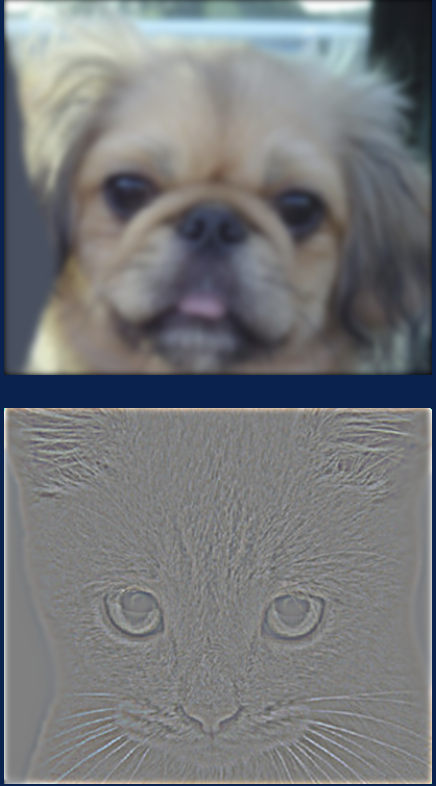
\includegraphics[width=0.3\textwidth]{imgs/pt3-1.png}

The result using different values of $\sigma$ are shown, this is for $sigma_{dog}=3$ and $\sigma_{cat}=6$:\\
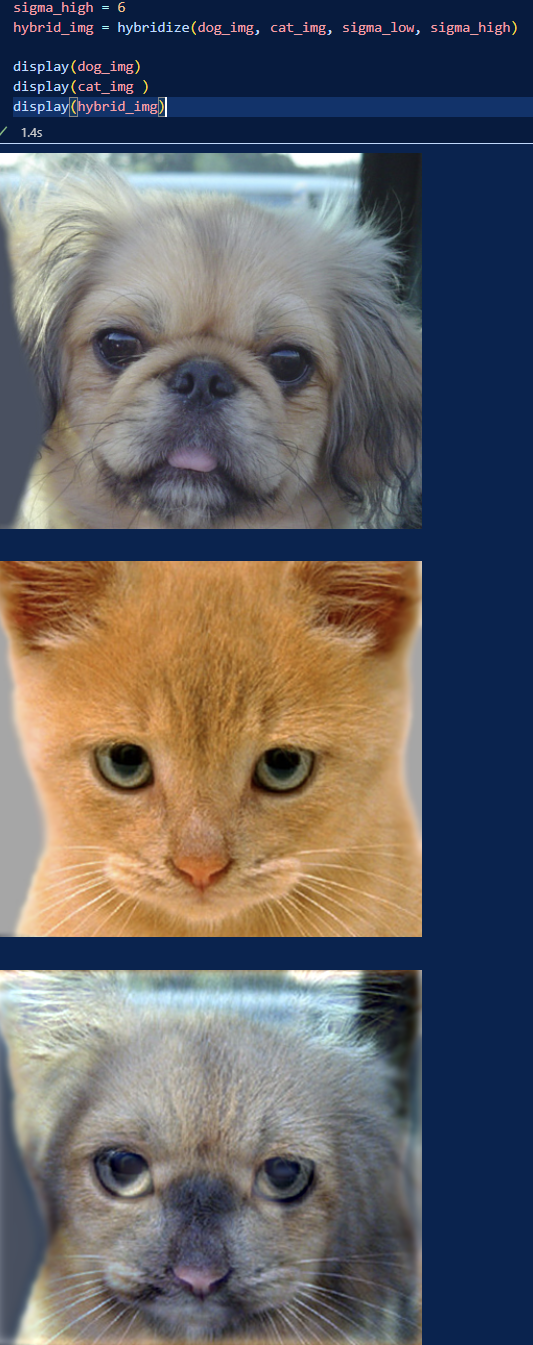
\includegraphics[width=0.3\textwidth]{imgs/pt3-2.png}
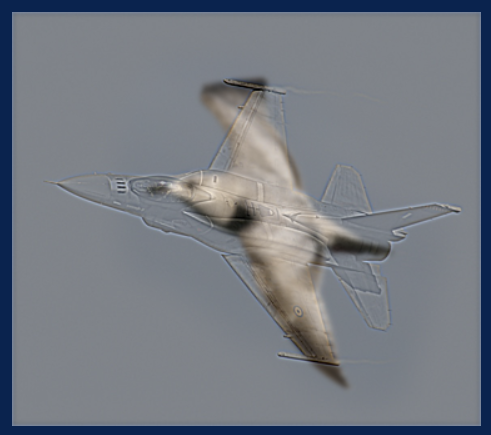
\includegraphics[width=0.3\textwidth]{imgs/pt3-3.png}

Other combinations have been tried but in the interest of time are not included in this report

\section*{Part 4}

The different blur techniques are shown. The speckeled is on the left, with Gaussian noise on the right:\\
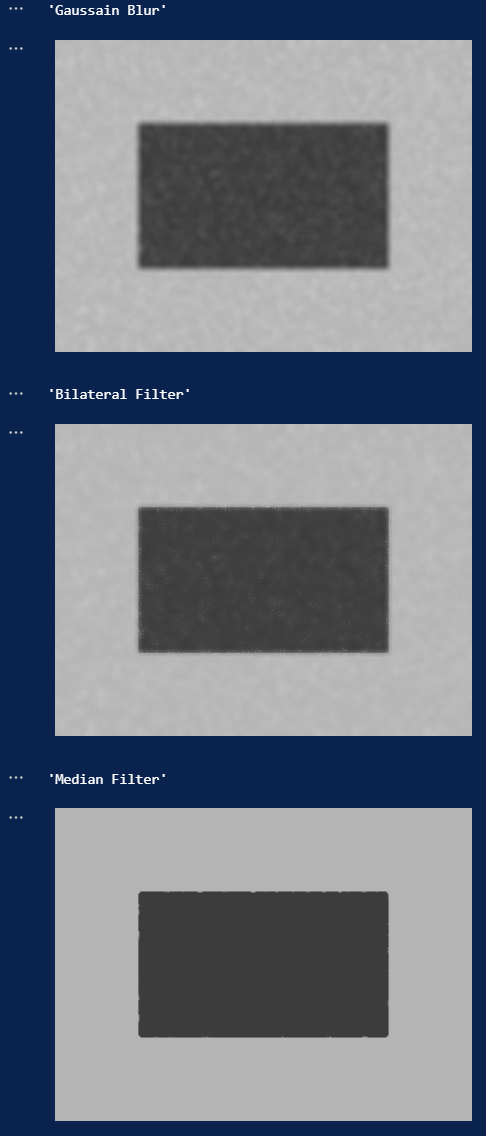
\includegraphics[height=\textwidth]{imgs/pt4-1.png}
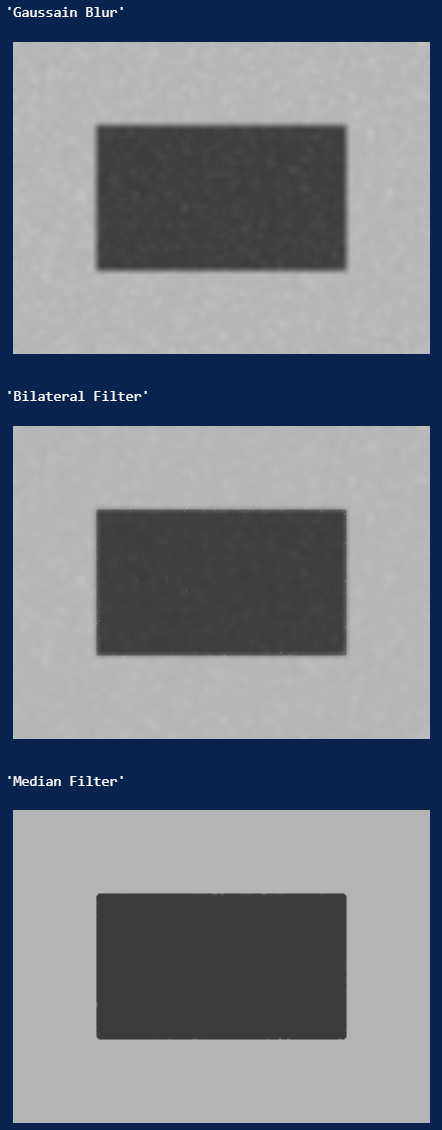
\includegraphics[height=\textwidth]{imgs/pt4-2.png}

\subsection*{2.}
The speckeled is on the left, with Gaussian noise on the right. Applying the specific filters yields:

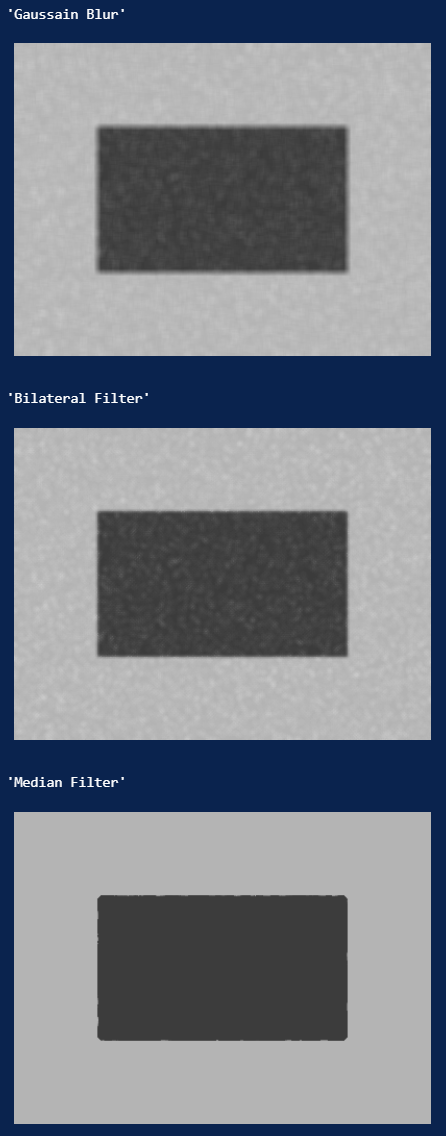
\includegraphics[height=\textwidth]{imgs/pt4-3.png}
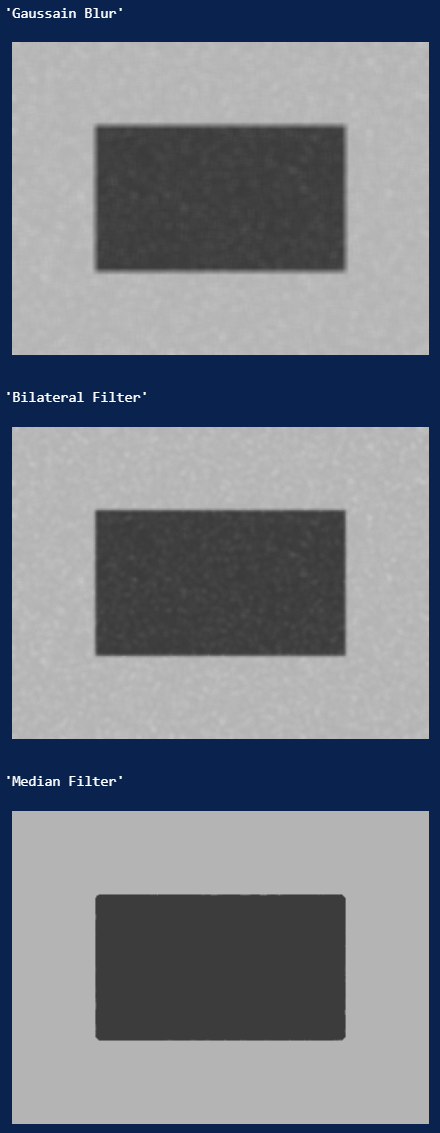
\includegraphics[height=\textwidth]{imgs/pt4-4.png}

There is some ringing that is observed in the top filter. This is showing up as squarish artifacts. It is because the Gaussian sigma value is so high compared to a the size of the filter that for all purposes it has become a simple box filter with all the same associated issues. It is worse on the speckled sample because it has more drastic pixel changing patterns that can induce this. Particularly prominanet is the edges of the dark inner rectangle when zoomed in.

The second set of images have a similar issue because the distance element is a box filter with large sigma. The 150 sigma in the color space however is still effectively Gaussian and so the ringing is not as severe around the dark rectangle, but still present. It has also helped filter speckles with fewer artifacts.

The median filters don't have the same artifacting as previous filters and appear to be the most effective of the three in recovering the original image. The speckeled image has more of a ragged edge.

Gaussian and bilateral will keep the original straight lines straigt, but at the cost of image artifacting, they are also sensitive to variance on the functions. The median filter is more robust but can result in rgged edges. The gaussian filters are more effective on white noise than on speckeled noise.

\end{document}